%%%%%%%%%%%%%%%%%%%%%%%%%%%%%%%%%%%%%%%%%%%%%%%%%%%%%%%%%%%%%%%%%%%%%%%%%%%%%%%%%%%%%%%%%%%%%%%%%%%%%%
%
%   Filename    : chapter_4.tex 
%
%   Description : This file will contain your System.
%                 
%%%%%%%%%%%%%%%%%%%%%%%%%%%%%%%%%%%%%%%%%%%%%%%%%%%%%%%%%%%%%%%%%%%%%%%%%%%%%%%%%%%%%%%%%%%%%%%%%%%%%%
\newcommand{\systemname}{FB Stories } 

\chapter\systemname
\label{sec:\systemname}

This chapter discusses the functional requirements and the overall specifications of the software developed as part of this research, called \systemname. It introduces the software, its objectives, scope and limitations, architecture, and features.

%section~~~~~~~~~~~~~~~~~~~~~~~~~~~~~~~~~~~~~~~~~~~~~~~~~~~~~~~~~~~~~~
\section{An Overview}
\systemname is a web-based application where Facebook users can generate their own life stories through the data gathered from their Facebook account, with the use of natural language processing (NLP) and generation (NLG) techniques. 

To use \systemname, the user must log in to their Facebook account to allow access to their data. The data extracted will be classified as either direct knowledge or indirect knowledge. For indirect knowledge, text understanding techniques will be applied. 

The software then proceeds to the text generation module, where it determines which elements of the extracted data are appropriate and can be used in generating the life story, and constructs corresponding story text from these data. Once the life story text has been generated, the user is given the option to save the story into a text file.

The completed life story contains three parts. The first part contains basic information or facts about the user. The second part contains data extracted from the Facebook posts that were classified and stored into the indirect knowledge base. The third part contains the list of preferences of the user inferred from the available list of page likes, as well as some recent events that this person has attended.

%section~~~~~~~~~~~~~~~~~~~~~~~~~~~~~~~~~~~~~~~~~~~~~~~~~~~~~~~~~~~~~~
\section{Software Objectives}
This section presents the general and specific objectives of \systemname.

\subsection{General Objective}
To generate a story that takes into account the Facebook posts of a user by using natural language processing techniques.

\subsection{Specific Objectives}
\begin{enumerate}
\item To extract needed data from Facebook;
\item To use data processing techniques to analyze the input; 
\item To classify each post according to its type;
\item To use text generation techniques to generate a story;
\item To allow users to save the generated stories into a text file.
\end{enumerate}

%section~~~~~~~~~~~~~~~~~~~~~~~~~~~~~~~~~~~~~~~~~~~~~~~~~~~~~~~~~~~~~~
\section{Scope and Limitations of the Software}

\subsection{Data Extraction}
In retrieving data from a user's Facebook account, asking for user's permission is necessary. A successful login to the user's Facebook account means that the user permits the system to make use of their data. These permissions will be readily set out for the user to approved, and once set, selected options cannot be altered. If the user does not allow the software to access his/her profile with the given permissions, only those public information and public posts of the user are extracted. 

\systemname does not extract data from Messenger, as well as information about the user's interactions (such as who Liked the user's posts).

\subsection{Data Processing}
Data processing techniques are only applicable to Facebook posts. The system does not perform any verification on the correctness of the user's  data.

Hashtags, hyperlinks, emoticons, laughter, and foreign characters are removed from posts before undergoing text understanding, in order to lessen misclassifications. For posts with mixed languages, abbreviations and incomplete sentences, the interpretation of these are limited by what the API can offer \figref{fig:MixedLanguage}. The syntax analysis returned by the tool is not checked for the correctness of its output. In \figref{fig:MixedLanguage}, ``kain” is a Filipino word which means ``eat”, thus it should be a verb not a noun. 

\begin{figure}[!htb]                %-- use [t] to place figure at top, [b] to place at the bottom, [h] for here
   \centering                    %-- use this to center the figure
   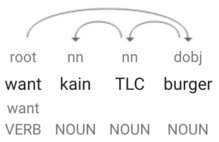
\includegraphics [width=2.5in,height=2.5in,keepaspectratio] {MixedLanguage.png}      %-- include image file named as "disneychart.png" 
   \caption{Sample Incomplete Text with Mixed Languages and Abbreviation.}
    \label{fig:MixedLanguage}
\end{figure}

\subsection{Post Classification}
Posts extracted from Facebook cannot be used directly in generating story text, since users tend to post snippets of incomplete, context-based data. Other posts have no explicit verbs used to describe the event. Thus, the posts must be individually processed to extract the necessary information comprising an event.

Although Facebook has a feature called \textit{Predefined Activities} to enable users to easily  classify their individual posts according to the content, there are currently no tools that can support the extraction of relevant elements from posts that uses this feature. Thus, a post classification algorithm is needed to classify each Facebook post as either \textit{celebrating} post, \textit{travelling} post, \textit{drinking} post, \textit{eating} post or \textit{no event} post. These four types of posts are chosen to be used in this research since majority of Facebook posts gathered and analyzed fall under them. Other types of posts such as \textit{reading}, \textit{listening}, \textit{watching}, among others may be present in the extracted Facebook posts, but will be ignored and will be tagged as \textit{no event} posts for this research.

\subsection{Text Generation}
Text generation has three components. One component is responsible for generating the introductory part of the story text, the second component is responsible for generating the body and the last component is responsible for generating the conclusion.

The introduction contains basic information directly extracted from the user's profile without going through further processing. The body part of the life story contains events: information which underwent processing and post classification. The conclusion part of the life story contains the likes and preferences of the user, as well as recent Facebook Events attended. 

\subsection{Save to Text File}
The user might want to cherish and read previously generated life stories in the future, making it important to have a method to save stories. Text files are only generated based on the user's instructions. Other file types than \textit{.txt} are not supported. After successfully saving the generated story into a text file, the user is solely responsible for the safekeeping and/or dissemination of the file.

For purposes of validating the output of \systemname and for future research, a copy of the generated life story is also stored as part of the output of this research. The user is properly informed of this. Anonymizing the data for future use is provided as an option for confidentiality

\clearpage
%section~~~~~~~~~~~~~~~~~~~~~~~~~~~~~~~~~~~~~~~~~~~~~~~~~~~~~~~~~~~~~~
\section{Architectural Design}
\figref{fig:AD} is a representation of the architecture design of \systemname. It is divided into three big parts: initialization, text understanding, and text generation.

A more detailed discussion of the different modules is written in Chapter 5 for both the initial version of the system as well as the latest version as of the time of writing.

\begin{figure}[!htb]                %-- use [t] to place figure at top, [b] to place at the bottom, [h] for here
   \centering                    %-- use this to center the figure
   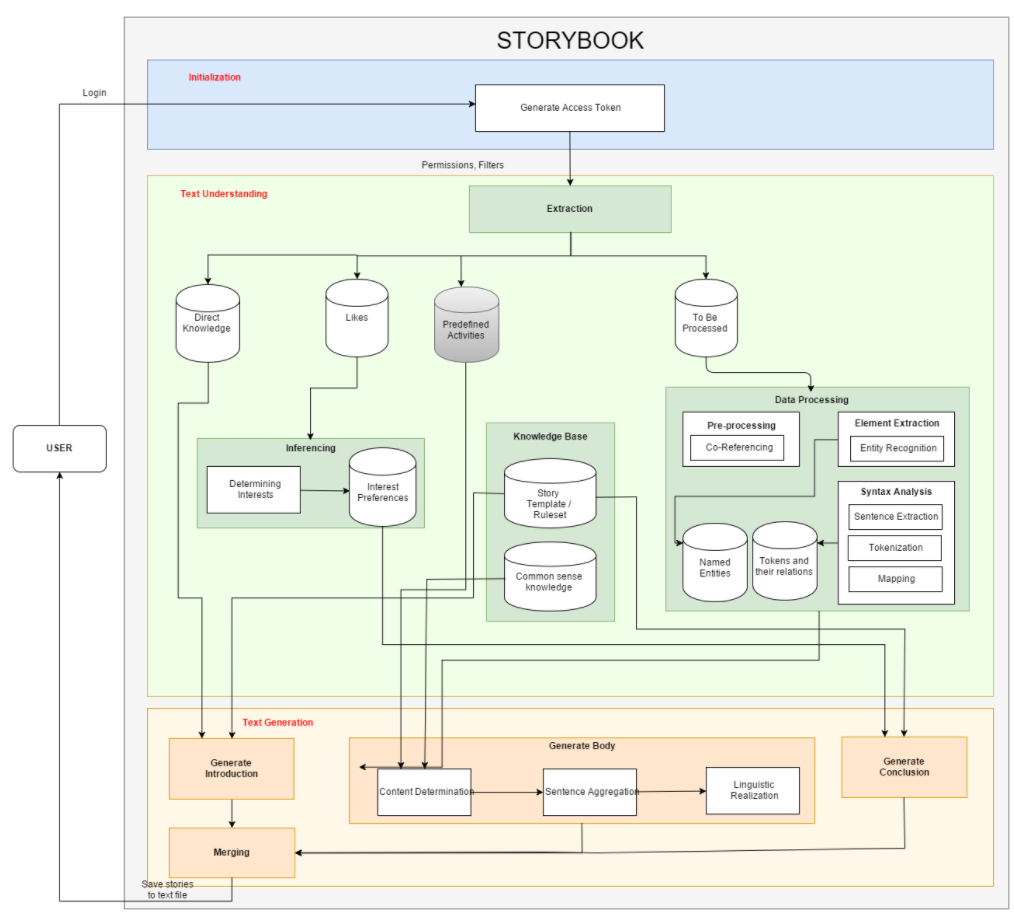
\includegraphics [width=\textwidth] {AD.png}      %-- include image file named as "disneychart.png" 
   \caption{Architecture Design of \systemname}
    \label{fig:AD}
\end{figure}

\subsection{Initialization}
Before the system can extract the user's data, it needs the user's permission, which the user grants by logging into Facebook and specifying that they agree with the data extraction to be done by FB Stories. After the user goes through each of the permissions and accepts it, Facebook generates an access token, which controls which data can be extracted by the data extraction tool.

The data extracted can be classified into one of three types:
\begin{itemize}
	\item \textit{Direct knowledge}. These are derived from the user's \textit{About Me} section, and are used for generating the introductory part of the life story.
	\item \textit{Data to be processed}. These are taken from the user's posts on their Timeline, and will be processed later on for use in generating the body.
	\item  \textit{User's list of Liked pages and Facebook Events}. These are derived from the user's account (Facebook keeps track of the user's list of Liked pages and Facebook Events attended). These will be used as part of the conclusion.
\end{itemize}

\subsection{Text Understanding}
For those data from which knowledge cannot be easily inferred, a more specific procedure of text understanding algorithms is applied. Data preprocessing processes the input in order to deal with issues present in user-generated data, such as stray characters or the presence of laughter. 

After preprocessing these data, they are then subjected to NLP processes which enable the system to figure out the relevant parts of these data to use in generating the story later on, such as who did what, what is being done, and to whom or to what. These data are then classified (with the help of the knowledge base) in order to figure out how they'll be organized in the final generated story. 

\subsection{Text Generation}
The text generation module is responsible for generating the appropriate story segments that make up the entire life story generated by FB Stories. There are three components: the \textit{GenIntro}, \textit{GenBody}, and \textit{GenConclusion}.

GenIntro uses data determined to be ``facts” or direct knowledge. It involves checking the knowledge base for the appropriate template to be used based on the available facts in the \textit{Direct Knowledge}, \textit{Educational Background}, \textit{Work}, and \textit{Family} table. GenIntro would also involve filling the template with the correct data. The generated text will become the introductory paragraph of the life story.

GenBody, on the other hand, is applied to generate the body of the life story from the data processed in the Data Processing module. The body paragraph(s) will be narrating one or more events about a person's life. These events will be taken from data that users have written and posted on their own Timeline. For these data, text generation is more complex. It will undergo three sub-modules, which are all detailed in Section 3.5.1, Text Generation.

GenConclusion will be used to generate the conclusion part of the story text, which will contain the user's likes and interested events. The exact process of determining the user's likes is explained in the Inferencing Section, 4.4.4. Similar to the approach in GenIntro, GenConclusion would check the available templates defined in the Template table and use the data stored in the \textit{Likes} and \textit{Events} table.

The generated texts from the three text generation modules are then merged, and presented to the user as the complete life story. The user will now have the option to save or discard their life story. If the user wishes to save their life stories, a text file will be created and the user chooses where to save this file. But if the user wishes to discard this, then they simply close the software.

%section~~~~~~~~~~~~~~~~~~~~~~~~~~~~~~~~~~~~~~~~~~~~~~~~~~~~~~~~~~~~~~
\section{Software Functions}
\systemname provides a simple environment that allows users to easily use it to create a life story from their Facebook posts and save these stories for future use. Below are the software functions used in \systemname.

\subsection{Login Window}
In using the application, the user would have to Login to Facebook for the software to access the data stored in his/her account. A Facebook login button would prompt the user to login as shown in \figref{fig:Login}. Once the button is clicked, a Login Window, which can be seen in \figref{fig:Login2}, would pop up informing the user that he/she is logging in his/her Facebook account with the app, StoryBook. Login information such as email address, phone number or user id along with the corresponding password are both needed to successfully login. 

Logging in to the app also grants the permissions set by the app which then automatically updates the access token stored in cookies. 

\begin{figure}[!htb]                %-- use [t] to place figure at top, [b] to place at the bottom, [h] for here
   \centering                    %-- use this to center the figure
   
\includegraphics [width=3in,height=2in,keepaspectratio] {login1.png}      %-- include image file named as "disneychart.png" 
   \caption{Facebook Login Button.}
    \label{fig:Login}
\end{figure}

\begin{figure}[!htb]                %-- use [t] to place figure at top, [b] to place at the bottom, [h] for here
   \centering                    %-- use this to center the figure
   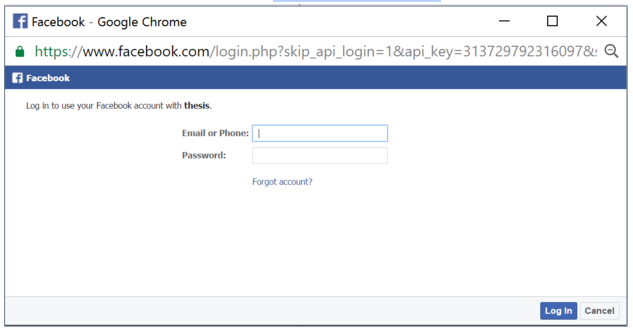
\includegraphics [width=\textwidth] {login2.png}      %-- include image file named as "disneychart.png" 
   \caption{Pop-up Login Window.}
    \label{fig:Login2}
\end{figure}

\subsection{Permission Window}
Logging in to Facebook automatically stores a default access token in cookies. If the user is already logged-in on Facebook and the \systemname automatically obtains the user's access token, then it would check permissions in the access token and prompts the user of the missing permissions it needs to acquire. \figref{fig:Permission} displays the permission window that asks the user to grant the permissions needed by the software.

\begin{figure}[!htb]                %-- use [t] to place figure at top, [b] to place at the bottom, [h] for here
   \centering                    %-- use this to center the figure
   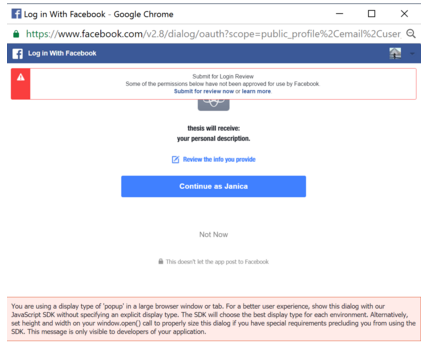
\includegraphics [width=\textwidth] {permission.png}      %-- include image file named as "disneychart.png" 
   \caption{Permission Window.}
    \label{fig:Permission}
\end{figure}

\subsection{Generated Story Output Window}
The Generated Story Output Window, \figref{fig:Output}, is basically a window that displays the generated story after \systemname has analyzed and processed the gathered data from the user's Facebook account. The user would be given an option to save the generated story to a text file through the ``Save to Text File" button.

\begin{figure}[!htb]                %-- use [t] to place figure at top, [b] to place at the bottom, [h] for here
   \centering                    %-- use this to center the figure
   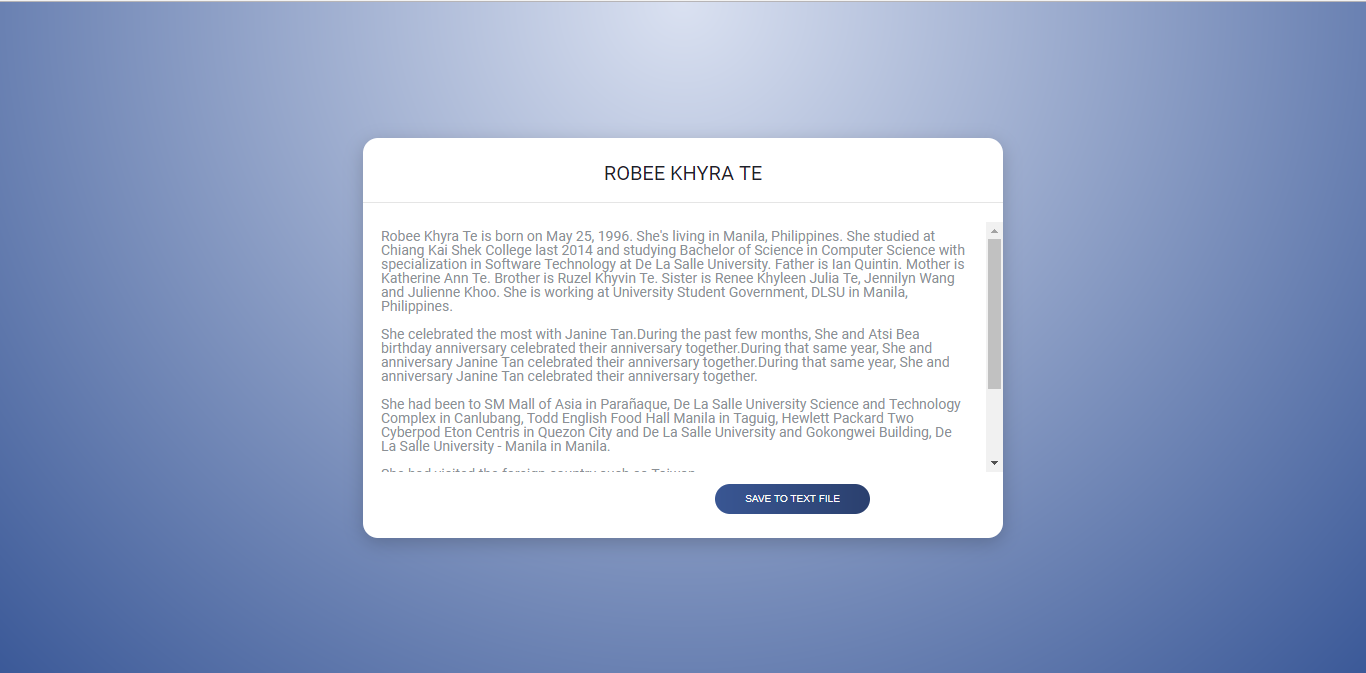
\includegraphics [width=\textwidth] {GeneratedStoryOutputWindow.png}      %-- include image file named as "disneychart.png" 
   \caption{Generated Story Output Window.}
    \label{fig:Output}
\end{figure}
\clearpage

\section{Physical Enviroment and Resources}
This section details the minimum and recommended software requirements for software implementation.

\systemname requires the following resources for development:
\begin{itemize}
\item Eclipse IDE
\item MySQL Server and Workbench
\item Java Development Kit (JDK)
\item Apache Tomcat 8.0
\end{itemize}

These are the minimum software requirements for \systemname to run properly:
\begin{itemize}
\item \textbf{OS}: Windows 8.1 / 10
\item \textbf{Memory}: 1 GB RAM
\item \textbf{Storage}: At most 1 GB of free hard disk space
\item \textbf{Internet connection}: Broadband, at least 1Mb/s bandwidth
\item \textbf{Others}: Java Runtime Environment (JRE), MySQL Server, Apache Tomcat 8.0
\end{itemize}

\subsection{Tools}
The following tools will be used for the development and runtime of the \systemname.

\subsubsection{Facebook Login API}
The Facebook Login API enables the use of the Facebook user's identity in order to craft interesting stories about them. It enables the application to extract data from Facebook to be processed and used to generate stories. Features of Facebook Login, such as access tokens and permissions, make it safe and secure for people and apps to use, but there are some security steps which this software will need to implement. This will be tackled in Chapter 5, Design and Implementation.

\subsubsection{Graph API}
The use of Graph API enables the software to extract posts and data from a specific Facebook account. It supports developers by supplying services such as providing snippets of codes for easier integration with JSON requests and responses.

\subsubsection{Stanford CoreNLP}
Stanford CoreNLP will be used in the text understanding module, as it provides the needed component, syntax analysis. 

\subsubsection{WordNet}
WordNet will be used to supply the data that is needed for the reference table which contains keywords such as related verbs and nouns. The reference table will then be used in the classification of Facebook post which does not contain a verb.

\subsubsection{ConceptNet}
ConceptNet is a semantic network containing concepts with Open Mind Common Sense as its main source of knowledge, along with other sources such as Wikipedia, WordNet, and DBPedia. This knowledge will be used to supply keywords for the reference table to be used in the post classification module. This will gather related verbs and noun for the categories \textit{Celebrating}, \textit{Travelling}, \textit{Eating}, and \textit{Drinking}.

\subsubsection{SimpleNLG}
SimpleNLG will be used in generating grammatically correct English sentences. SimpleNLG will also automate some of the tasks an NLG system needs to perform like checking the orthography, morphology and simple grammar of the sentences.